%% ----------------------------------------------------------------
%% Project.tex
%% ----------------------------------------------------------------
\documentclass[openany]{ecsproject}     % Use the Project Style
\graphicspath{{images/}}   % Location of your graphics files
%\DeclareGraphicsExtensions{.png,.jpg}
\usepackage[square,numbers]{natbib}            % Use Natbib style for the refs.
\hypersetup{colorlinks=true}   % Set to false for black/white printing
%% ----------------------------------------------------------------
%% Definitions.tex
%% ---------------------------------------------------------------- 
\newcommand{\BibTeX}{{\rm B\kern-.05em{\sc i\kern-.025em b}\kern-.08em T\kern-.1667em\lower.7ex\hbox{E}\kern-.125emX}}

%% People
\newcounter{address}
\setcounter{address}{1}
\renewcommand{\theaddress}{\textsuperscript{\fnsymbol{address}}}
\newcommand{\address}[1]{\refstepcounter{address}\theaddress#1\\}
\newcommand{\Name}[3]{\texorpdfstring{\href{mailto:#3}{#2}#1}{#2}\xspace}
\newcommand{\SteveRGunn}[1]{\Name{#1}{Steve R. Gunn}{S.R.Gunn@ecs.soton.ac.uk}}

%% Dingbats
\newcommand{\tick}{\ding{51}}
\newcommand{\cross}{\ding{55}}

%% Calculus
\newcommand{\pd}[2]{\ensuremath{\frac{\partial #1}{\partial #2}}\xspace}
\newcommand{\fd}[2]{\ensuremath{\frac{d #1}{d #2}}\xspace}
\newcommand{\dint}{\ensuremath{\int\!\!\!\int}\xspace}
\newcommand{\tint}{\ensuremath{\int\!\!\!\int\!\!\!\int}\xspace}

%% Math Sets
\newcommand{\Q}[1]{\ensuremath{\mathbb{#1}}\xspace}
\newcommand{\R}{\Q{R}}

%% Matrix, Vector
\newcommand{\V}[1]{\ensuremath{\boldsymbol{#1}}\xspace}
\newcommand{\M}[1]{\ensuremath{\boldsymbol{#1}}\xspace}
\newcommand{\0}{\V{0}}
\newcommand{\1}{\V{1}}
\newcommand{\I}{\M{I}}

%% Math Functions
\newcommand{\F}[1]{\ensuremath{\mathrm{#1}}\xspace}
\newcommand{\sgn}{\F{sgn}}
\newcommand{\tr}{\F{trace}}
\newcommand{\diag}{\F{diag}}

%% Math Names
\newcommand{\N}[1]{\ensuremath{\mathit{#1}}\xspace}

%% Data
\newcommand{\mc}[1]{\ensuremath{\mathcal{#1}}\xspace}
\newcommand{\Hyp}{\mc{H}}
\newcommand{\D}{\mc{D}}

%% Kernel
\newcommand{\K}{\M{K}}
\newcommand{\eins}{\texorpdfstring{\ensuremath{\epsilon}}{\textepsilon}-insensitive\xspace}
\newcommand{\e}{\ensuremath{\epsilon}\xspace}
\newcommand{\Bxi}{\ensuremath{\boldsymbol{\xi}}\xspace}
\newcommand{\Kanova}{\ensuremath{\mathit{K_{ANOVA}}}\xspace}
\newcommand{\Kspline}{\ensuremath{\mathit{K_{spline}}}\xspace}

%% Bayesian
\newcommand{\MP}{\ensuremath{\mathit{{\scriptscriptstyle \hspace{-1.5pt}M\hspace{-1.5pt}P}}}\xspace}
\newcommand{\ML}{\ensuremath{\mathit{{\scriptscriptstyle \hspace{-1.5pt}M\hspace{-1.5pt}L}}}\xspace}
\newcommand{\Qw}{\ensuremath{Q_{\w}(\w)}\xspace}
\newcommand{\Qa}{\ensuremath{Q_{\Ba}(\Ba)}\xspace}
\newcommand{\Qb}{\ensuremath{Q_{\beta}(\beta)}\xspace}
\newcommand{\wMPab}{\ensuremath{\w_{\MP|\bar {\Ba},\bar \beta}}\xspace}
\newcommand{\wMP}{\ensuremath{\w_{\MP}}\xspace}
\newcommand{\yMP}{\ensuremath{y_{\MP}}\xspace}
\newcommand{\BaMP}{\ensuremath{\Ba_{\hspace{1pt}\MP}}\xspace}
\newcommand{\aMP}{\ensuremath{\alpha_{\hspace{1pt}\MP}}\xspace}
\newcommand{\bMP}{\ensuremath{\beta_{\hspace{1pt}\MP}}\xspace}
\newcommand{\Sab}{\ensuremath{\M{\Sigma}_{\bar \Ba,\bar \beta}}\xspace}
\newcommand{\Ba}{\ensuremath{\boldsymbol{\alpha}}\xspace}
\newcommand{\Bb}{\ensuremath{\boldsymbol{\beta}}\xspace}
\newcommand{\Bm}{\ensuremath{\boldsymbol{\mu}}\xspace}
\newcommand{\BL}{\ensuremath{\boldsymbol{\Lambda}}\xspace}
\newcommand{\BPhi}{\ensuremath{\boldsymbol{\Phi}}\xspace}
\newcommand{\SMP}{\ensuremath{\M{\Sigma}_{\MP}}\xspace}

\newcommand{\Pa}{\ensuremath{P(\alpha|\mathcal{H})}\xspace}
\newcommand{\Pb}{\ensuremath{P(\beta|\mathcal{H})}\xspace}
\newcommand{\Pab}{\ensuremath{P(\alpha,\beta|\mathcal{H})}\xspace}
\newcommand{\Pw}{\ensuremath{P(\w|\mathcal{H})}\xspace}
\newcommand{\PD}{\ensuremath{P(\D|\mathcal{H})}\xspace}
\newcommand{\PwIa}{\ensuremath{P(\w|\alpha,\mathcal{H})}\xspace}
\newcommand{\PDIwb}{\ensuremath{P(\D|\w,\beta,\mathcal{H})}\xspace}
\newcommand{\PDwab}{\ensuremath{P(\D,\w,\alpha,\beta|\mathcal{H})}\xspace}
\newcommand{\PDIw}{\ensuremath{P(\D|\w,\mathcal{H})}\xspace}
\newcommand{\PwID}{\ensuremath{P(\w|\D,\mathcal{H})}\xspace}
\newcommand{\PwabID}{\ensuremath{P(\w,\alpha,\beta|\D,\mathcal{H})}\xspace}

\newcommand{\PanH}{\ensuremath{P(\alpha)}\xspace}
\newcommand{\PbnH}{\ensuremath{P(\beta)}\xspace}
\newcommand{\PabnH}{\ensuremath{P(\alpha,\beta)}\xspace}
\newcommand{\PwnH}{\ensuremath{P(\w)}\xspace}
\newcommand{\PDnH}{\ensuremath{P(\D)}\xspace}
\newcommand{\PwIanH}{\ensuremath{P(\w|\alpha)}\xspace}
\newcommand{\PDIwbnH}{\ensuremath{P(\D|\w,\beta)}\xspace}
\newcommand{\PDwabnH}{\ensuremath{P(\D,\w,\Ba,\beta)}\xspace}
\newcommand{\PDIwnH}{\ensuremath{P(\D|\w)}\xspace}
\newcommand{\PwIDnH}{\ensuremath{P(\w|\D)}\xspace}
\newcommand{\PwabIDnH}{\ensuremath{P(\w,\alpha,\beta|\D)}\xspace}

\newcommand{\PDwBab}{\ensuremath{P(\D,\w,\Ba,\beta|\mathcal{H})}\xspace}
\newcommand{\PwIBa}{\ensuremath{P(\w|\Ba,\mathcal{H})}\xspace}
\newcommand{\PBab}{\ensuremath{P(\Ba,\beta|\mathcal{H})}\xspace}
\newcommand{\PwBabID}{\ensuremath{P(\w,\Ba,\beta|\D,\mathcal{H})}\xspace}

\newcommand{\PBanH}{\ensuremath{P(\Ba)}\xspace}
\newcommand{\PwIBanH}{\ensuremath{P(\w|\Ba)}\xspace}

%% Snakes
\newcommand{\Esnake}{\ensuremath{\mathit{E_{snake}}}\xspace}
\newcommand{\Eimage}{\ensuremath{\mathit{E_{image}}}\xspace}
\newcommand{\Econt}{\ensuremath{\mathit{E_{cont}}}\xspace}
\newcommand{\Ecurv}{\ensuremath{\mathit{E_{curv}}}\xspace}
\newcommand{\Eint}{\ensuremath{\mathit{E_{int}}}\xspace}
\newcommand{\Eext}{\ensuremath{\mathit{E_{ext}}}\xspace}
\newcommand{\Eterm}{\ensuremath{\mathit{E_{term}}}\xspace}
\newcommand{\Eline}{\ensuremath{\mathit{E_{line}}}\xspace}
\newcommand{\Eedge}{\ensuremath{\mathit{E_{edge}}}\xspace}
\newcommand{\Econ}{\ensuremath{\mathit{E_{con}}}\xspace}
\newcommand{\Eangle}{\ensuremath{\mathit{E_{angle}}}\xspace}
\newcommand{\Elshape}{\ensuremath{\mathit{E_{lshape}}}\xspace}
\newcommand{\Eedgedir}{\ensuremath{\mathit{E_{edgedir}}}\xspace}
\newcommand{\Emodel}{\ensuremath{\mathit{E_{model}}}\xspace}
\newcommand{\wte}{\ensuremath{\mathit{w_{term}}}\xspace}
\newcommand{\wli}{\ensuremath{\mathit{w_{line}}}\xspace}
\newcommand{\wed}{\ensuremath{\mathit{w_{edge}}}\xspace}
\newcommand{\wco}{\ensuremath{\mathit{w_{con}}}\xspace}

%% Environments
\newcounter{alg}
\newenvironment{algorithm}[1]
{
    \stepcounter{alg}
    \begin{table}[htb]
    \centering
    \begin{tabular}[t]{ll}
    \hline&\\
    \multicolumn{2}{l}{\bf Algorithm \arabic{alg}: #1}\\&\\
} {
    &\\
    \hline
    \end{tabular}
    \end{table}
}
            % Include your abbreviations
%\bibliographystyle{ecs}
\bibliographystyle{ieeetr}
%% ----------------------------------------------------------------
\begin{document}
\frontmatter
\title      {Energy efficient object detection and tracking through adaptive operation on heterogeneous multi-core systems}
\authors    {\texorpdfstring
             {\href{mailto:yz39g13@soton.ac.uk}{Yubo Zhi}}
             {Yubo Zhi}
            }
\addresses  {\groupname\\\deptname\\\univname}
\date       {\today}
\subject    {}
\keywords   {}
\supervisor {\texorpdfstring
             {\href{mailto:gvm@ecs.soton.ac.uk}{Dr Geoff Merrett}}
             {Yubo Zhi}
	    }
\examiner   {\texorpdfstring
             {\href{mailto:example@soton.ac.uk}{Someone}}
             {Someone}
	    }
\degree     {BEng Electronic Engineering}
\maketitle

\begin{abstract}
Object detection and tracking is a key technique used in computer vision applications, especially robotic systems, artificial intelligence and video surveillance systems, but video processing algorithms require a lot of computations, consume a significant amount of energy. This project was purposed to reduce power consumption and possibly improves performance of camera based real-time object detection and tracking applications. Such an application may rely heavily on battery power or harvesting energy from environment, hence power consumption on those devices becomes critical. As battery technology development was not as fast as electronic processing technology development, lower power consumption implies longer battery life for mobile devices e.g. laptops and smart phones, also lower environmental impact.

This project investigated some hardware based methodologies to achieve an overall reduction of computations required for doing continuous real-time object detection and tracking, includes dynamical control of hardware downsampling and cropping provided by the camera controller, automatic camera sleeping and frame rate reduction based on whether objects detected, their location and moving speed relative to the camera sense.

\iffalse
The implementations and investigations were hosted on the NVIDIA Tegra K1 embedded platform, features a GPU accelerated OpenCV library, .



In order to achieve this, automatic feedback control need to be developed based on previously recorded moving objects positions and velocities. GPU accelerated computer vision algorithm will also be deployed to minimise power consumption and computation time. For easier power consumption analysis, the Jetson embedded development platform featuring a quad-core ARM CPU and a CUDA-enabled Tegra GPU, introduced by NVIDIA, will be used in this project.

In technical aspect, OpenCV API for Tegra with CUDA GPU acceleration developed by NVIDIA for the embedded platform will be used to implement the video processing algorithm. The algorithm will employ the widely used background subtraction technique to detect foreground moving objects and get their coordinates. A camera will also be interfaced with the platform to do capturing and detecting objects in real-time, by a Linux kernel module driver. Afterwards, an automatic feedback frame rate and resolution control will be implemented, then power consumption with different operation modes will be investigated and the energy saved by applying the proposed method will be analysed.

If time allows, object identification may also be implemented, and possibly power saving technique will be investigated.

The aims of this project are:
	(internet enabled?)
Implement: // Using CUDA / OpenCV on Jetson
	Detect car in image
	Potentially track through series of images
Adaptive operation / optimise for energy: // Measurement & testing
	Improve energy efficiency by reduce frame rate when detected vehicle speed is slow
	Change image resolution
\fi
\end{abstract}

\tableofcontents
%\listoffigures
%\listoftables
%\lstlistoflistings
%\listofsymbols{ll}{$w$ & The weight vector}

%\acknowledgements{Thanks to no one.}
%\dedicatory{To \dots}
\mainmatter

%% ----------------------------------------------------------------
%% ----------------------------------------------------------------
%% Goal.tex
%% ----------------------------------------------------------------
\chapter{Project Goals} \label{Chapter:Goals}

\section{The problem}

With the rapid growth of integrated circuit manufacture technology, processing power was just enough to realise computation intensive computer vision algorithms by a small form factor mobile device. Such a battery powered mobile device provides considerable flexibility and is an essential part in robotic systems, artificial intelligence and machine learning. However, mobile devices generally have limited processing power, memory, storage and energy, but video processing algorithms involves lots of computations, hence could be the most power intensive and time consuming part in such application.

\section{Aims}

The aim of this project was to investigate ways to reduce overall power consumption of camera based real-time object detection and tracking applications, by applying feedback control of the camera module based on previous tracking results and utilising existing camera hardware capabilities including downsampling and cropping instead of software algorithms, while keeping a sensible accuracy. By doing so the average computation time would be dramatically reduced, hence reducing the overall power consumption.

The targets to be achieved are:

\begin{itemize}
  \item Development of a basic object tracking system, identify algorithms suitable for real-time operation, minimise operating system overheads.
  \item Interfacing camera module with the embedded system, expose control functions.
  \item Develop and analyse automatic camera frame rate reduction.
  \item Develop and analyse hardware downsampling and cropping.
  \item If time allows, object recognition may be implemented.
\end{itemize}

\chapter{Background and literature search}

There are lots of different algorithms and approaches existing in the field of object detection and tracking. Some of those algorithms were investigated in this project in order to identify a set of suitable algorithms that were both accurate and efficient enough to \moda{analyse} video stream from \mdc{a camera} by an embedded platform in real time.

Object tracking typically consists of 2 steps. Initially, locations and shapes of each moving object appeared in each frame need to be identified. Subsequently, by analysing and recording the movements of each object in sequential frames, the objects in a video stream can be tracked.

\section{OpenCV computer vision library}

% {\color{red}Information...}

OpenCV computer vision library \cite{opencv} is a very powerful open-source computer vision library. \moda{It contains lots of useful computer vision algorithms designed for computational efficiency and real-time applications. It is also mostly platform independent \mdc{enabling} easy platform adaptation. Furthermore, it can take the advantage of multi-core and GPU parallel processing on heterogeneous platforms by using a dedicated GPU algorithm module.}

\section{Model based object detection algorithms}

\iffalse
Being able to detect objects in a video frame is the first, also the most important and challenging step to do object tracking. This is generally accomplished by separation of foreground objects and background image.
\fi

Object detection is generally accomplished by separation of foreground and background masks, called background subtraction or foreground segmentation.

\subsection{Colour based}
\label{bgs:colour}

\mdc{Colours} can sometimes provide enough information about a specific object, \mdc{such as} a coloured ball. For filtering a specific colour out from a video frame, hue-saturation-value (HSV) colour space \cite[p.~301]{colourspace} representation is usually used, which can make colour filtering a lot easier based on hue, saturation and brightness information of the specific colour. In this way, a foreground mask can be generated easily by filtering \mdc{the} target colour. For example, \fref{Figure:MOTBOC} shows a simple colour filtering object detection implementation \cite{MOTBOC.git} that is able to detect objects with specific colours.

\begin{figure}[H]
  \centering
  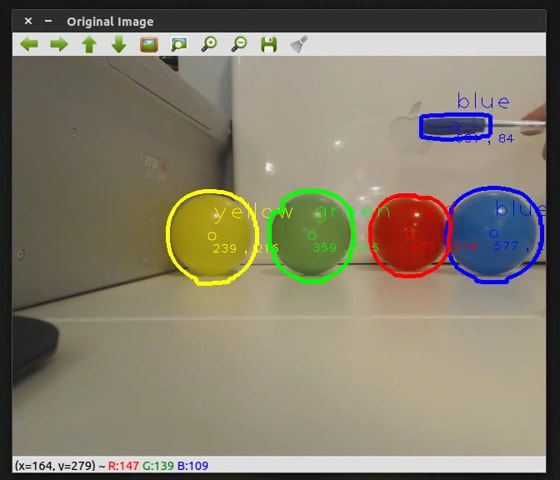
\includegraphics[width=0.5\columnwidth]{MOTBOC}
  \caption{Multi object tracking based on colour filtering (sourced from \cite{MOTBOC.git}).}
  \label{Figure:MOTBOC}
\end{figure}

This implementation does not require a lot of graphic processing, thus can be very quick and efficient, suitable for robots that are tracking something like a coloured ball or \mdc{a} piece of paper, \mdc{it} also could be useful for line racing car projects.

There are also researches using a more complex particle filtering algorithm based on colour distributions over a region in the frame \cite{nummiaro2003color}\mdc{. The results are shown in} \fref{Figure:nummiaro2003color}. \mdc{Firstly the cameras need to be calibrated and compensated. Then} a colour distribution model of the target object \mdc{needs} to be built\mdc{. Followed by that,} the elliptical region of the tracked object get determined by \mdc{applying} colour-based particle filters \cite{nummiaro2003adaptive}. The algorithm from the research are purposed to be used in multi-camera environments to select the best view of the target, therefore several views from different \mdc{cameras} are shown by the images at the bottom, along with the coefficients \mdc{implying the} similarity with the target model shown at the top left, and the selected best view at the top right.
% {\color{red}Details on algorithm implementation required.}

\begin{figure}[H]
  \centering
  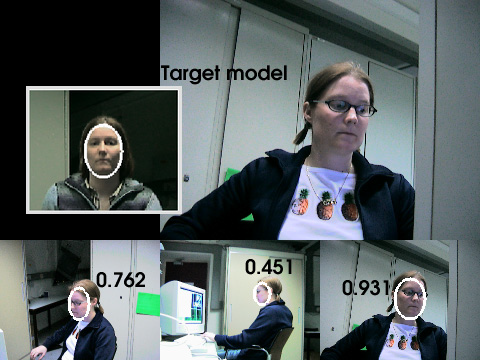
\includegraphics[width=0.5\columnwidth]{nummiaro2003color}
  \caption{Object tracking based on colour distribution particle filtering in multi-camera environments (sourced from \cite{nummiaro2003color}).}
  \label{Figure:nummiaro2003color}
\end{figure}

However, if there were other targets with \mdc{a} similar colour distribution, the algorithm \modc{might fail} to distinguish them, as shown \mdc{in} the second image in \fref{Figure:nummiaro2003color_fail}, the face of the man got tracked instead of the target woman's face. It also requires a specific model associated with each of the objects to be tracked.

\begin{figure}[H]
  \centering
  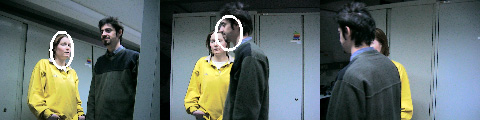
\includegraphics[width=0.9\columnwidth]{nummiaro2003color_fail}
  \caption{Problems on colour based object tracking, when several good candidates exists at the same time (sourced from \cite{nummiaro2003color}).}
  \label{Figure:nummiaro2003color_fail}
\end{figure}

\subsection{Shape matching}

Another important information about an object might be its distinctive shape. By extracting object edges in the scene \modc{and} apply appropriate shape matching algorithms, an object can be detected based on its shape.

This research \cite{borovicka2003circle} shows the ability to detect circles in a image by applying edge filtering followed by Hough \moda{transform}, as shown \mdc{in} \fref{Figure:circles}. \fref{Figure:circle:original} shows the original grey scaled image, then after blurred and Sobel filtered (\fref{Figure:circle:sobel}), clear edges \mdc{can be} extracted (\fref{Figure:circle:edge}). Finally, Hough transform \mdc{is} applied, the results merged with the original image are shown \mdc{in} \fref{Figure:circle:circles}.

\begin{figure}[H]
  \centering
  \subfigure [] {
    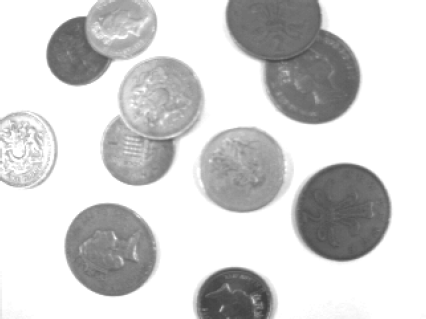
\includegraphics[width=0.22\columnwidth]{circle_original}
    \label{Figure:circle:original}
  }
  \subfigure [] {
    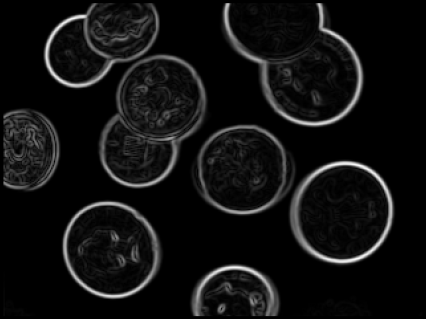
\includegraphics[width=0.22\columnwidth]{circle_sobel}
    \label{Figure:circle:sobel}
  }
  \subfigure [] {
    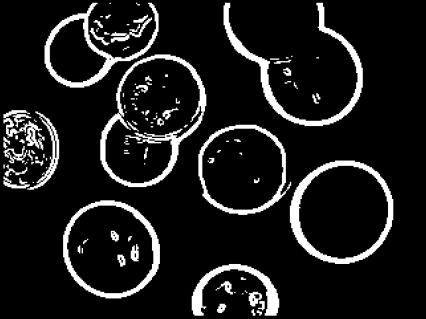
\includegraphics[width=0.22\columnwidth]{circle_edge}
    \label{Figure:circle:edge}
  }
  \subfigure [] {
    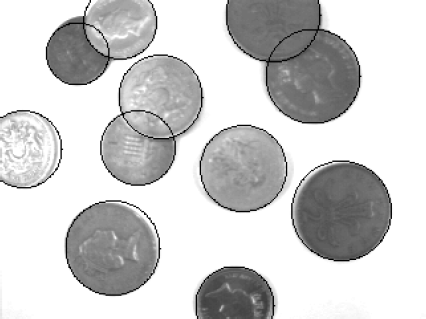
\includegraphics[width=0.22\columnwidth]{circle_circles}
    \label{Figure:circle:circles}
  }
  \caption{Circle detection by Hough transform (sourced from \cite{borovicka2003circle}). \subref{Figure:circle:original} shows the original image, \subref{Figure:circle:sobel} Sobel filters applied, \subref{Figure:circle:edge} threshold edge map, \subref{Figure:circle:circles} detected circles}
  \label{Figure:bg_circles}
\end{figure}

This implementation might be suitable for ball tracking \mdc{purposes}. By combining with the colour filtering as described in Section \ref{bgs:colour}, a single coloured ball could be efficiently tracked.

\subsection{Feature detection (Cascade classifier)}
\label{sec:bg:cc}

% {\color{red}Use this: \cite{viola2001rapid}}

Cascade classifier \cite{cascade} \cite{viola2001rapid} is a widely used object detection technique based on machine learning. By concatenating a large number of simple feature detectors (i.e. classifiers) each detecting different simple features based on \mdc{the} intensity at different positions as shown \mdc{in} \fref{bg:cc}, complex objects such as human faces can be recognised as shown in \moda{\fref{bg:cc:faces}}. Furthermore\mdc{,} its accuracy can be improved by training the classifier both positively and negatively.

\begin{figure}[H]
  \centering
  \subfigure [] {
    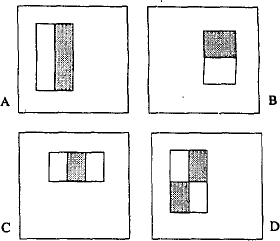
\includegraphics[width=0.3\columnwidth]{cc_features}
    \label{bg:cc:features}
  }
  \subfigure [] {
    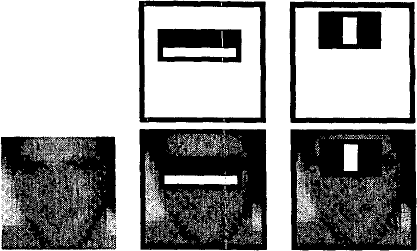
\includegraphics[width=0.3\columnwidth]{cc_face}
    \label{bg:cc:face}
  }
  \caption{Cascade classifier (sourced from \cite{borovicka2003circle}). \subref{bg:cc:features} shows some example simple feature detector configurations, \subref{bg:cc:face} shows some feature detector used on face recognition.}
  \label{bg:cc}
\end{figure}

\begin{figure}[H]
  \centering
  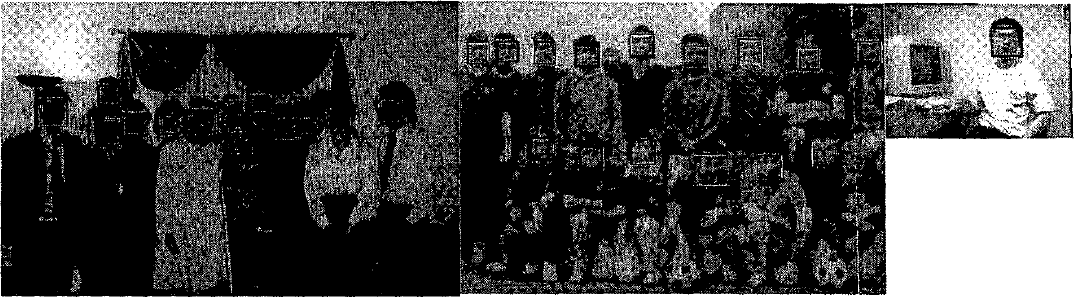
\includegraphics[width=0.9\columnwidth]{cc_faces}
  \caption{Cascade classifier recognising human faces (sourced from \cite{borovicka2003circle}).}
  \label{bg:cc:faces}
\end{figure}

This algorithm is mostly used for object classification, \mdc{such as} recognising human faces, bodies and different classes of vehicles in images. Like other \mdc{model-based} algorithms, multiple classifier definitions are required for detecting different kinds of objects, or even different perspectives of the same object.

% {\color{red}Replace with results from research paper}

\section{Motion-based object detection algorithms}

\subsection{Background subtraction}
\label{motion_bs}

By studying frames from a video stream then \mdc{building} up a background model image, it is also possible to detect moving objects in following frames efficiently.

% {\color{red}Add some graph from research paper?}

% {\color{red}Should be in design section?

% This type of algorithms suit well for static camera movement tracking, and were not limited by objects' geometry shapes, therefore was used in this project.}

% {\color{cyan}Background subtraction algorithms:

There are several background subtraction algorithms available, the BGSLibrary \cite{bgslibrary} is specifically developed for \mdc{analysing} those algorithms, it offers 37 different background subtraction algorithms implemented \mdc{by} OpenCV, published under GNU GPL v3 license. With the same programming interface for all available algorithms, it allows easy swapping between algorithms.

There is an article \cite{bgs:article} reviewed the algorithms available in the BGSLibrary, ranked \mdc{top 5 algorithms} in overall performance score as shown in \tref{Table:bgs}. \fref{bgsreview} shows foreground masks obtained from the top 5 algorithms on sequences from real world videos at the same frame. \moda{TP pixels indicate foreground pixels classified as foreground, and TN pixels indicate background pixels classified as background. Both TP and TN pixels combined \mdc{together} are the expected results, named ground truth foreground masks. FP pixels indicate background pixels classified as foreground, and FN pixels indicate foreground pixels classified as background. Both FP and FN pixels are incorrect results produced by the algorithm.} The actual foreground masks generated by the algorithms are TP and FN pixels.

\begin{table}[H]
  \centering
  \begin{tabular}{cc}
  \toprule
  \textbf{Method ID} & \textbf{Method name}\\
  \midrule
  PBAS & Pixel-Based Adaptive Segmenter \\
  MultiLayerBGS & Multi-Layer BGS \\
  MixtureOfGaussianV1BGS & Gaussian Mixture Model \\
  LBAdaptiveSOM & Adaptive SOM \\
  DPWrenGABGS & Gaussian Average \\
  \bottomrule
  \end{tabular}
  \caption{Background substraction algorithms investigated (adapted from \cite{bgslibrary})}
  \label{Table:bgs}
\end{table}

\begin{figure}[tbh]
  \centering
  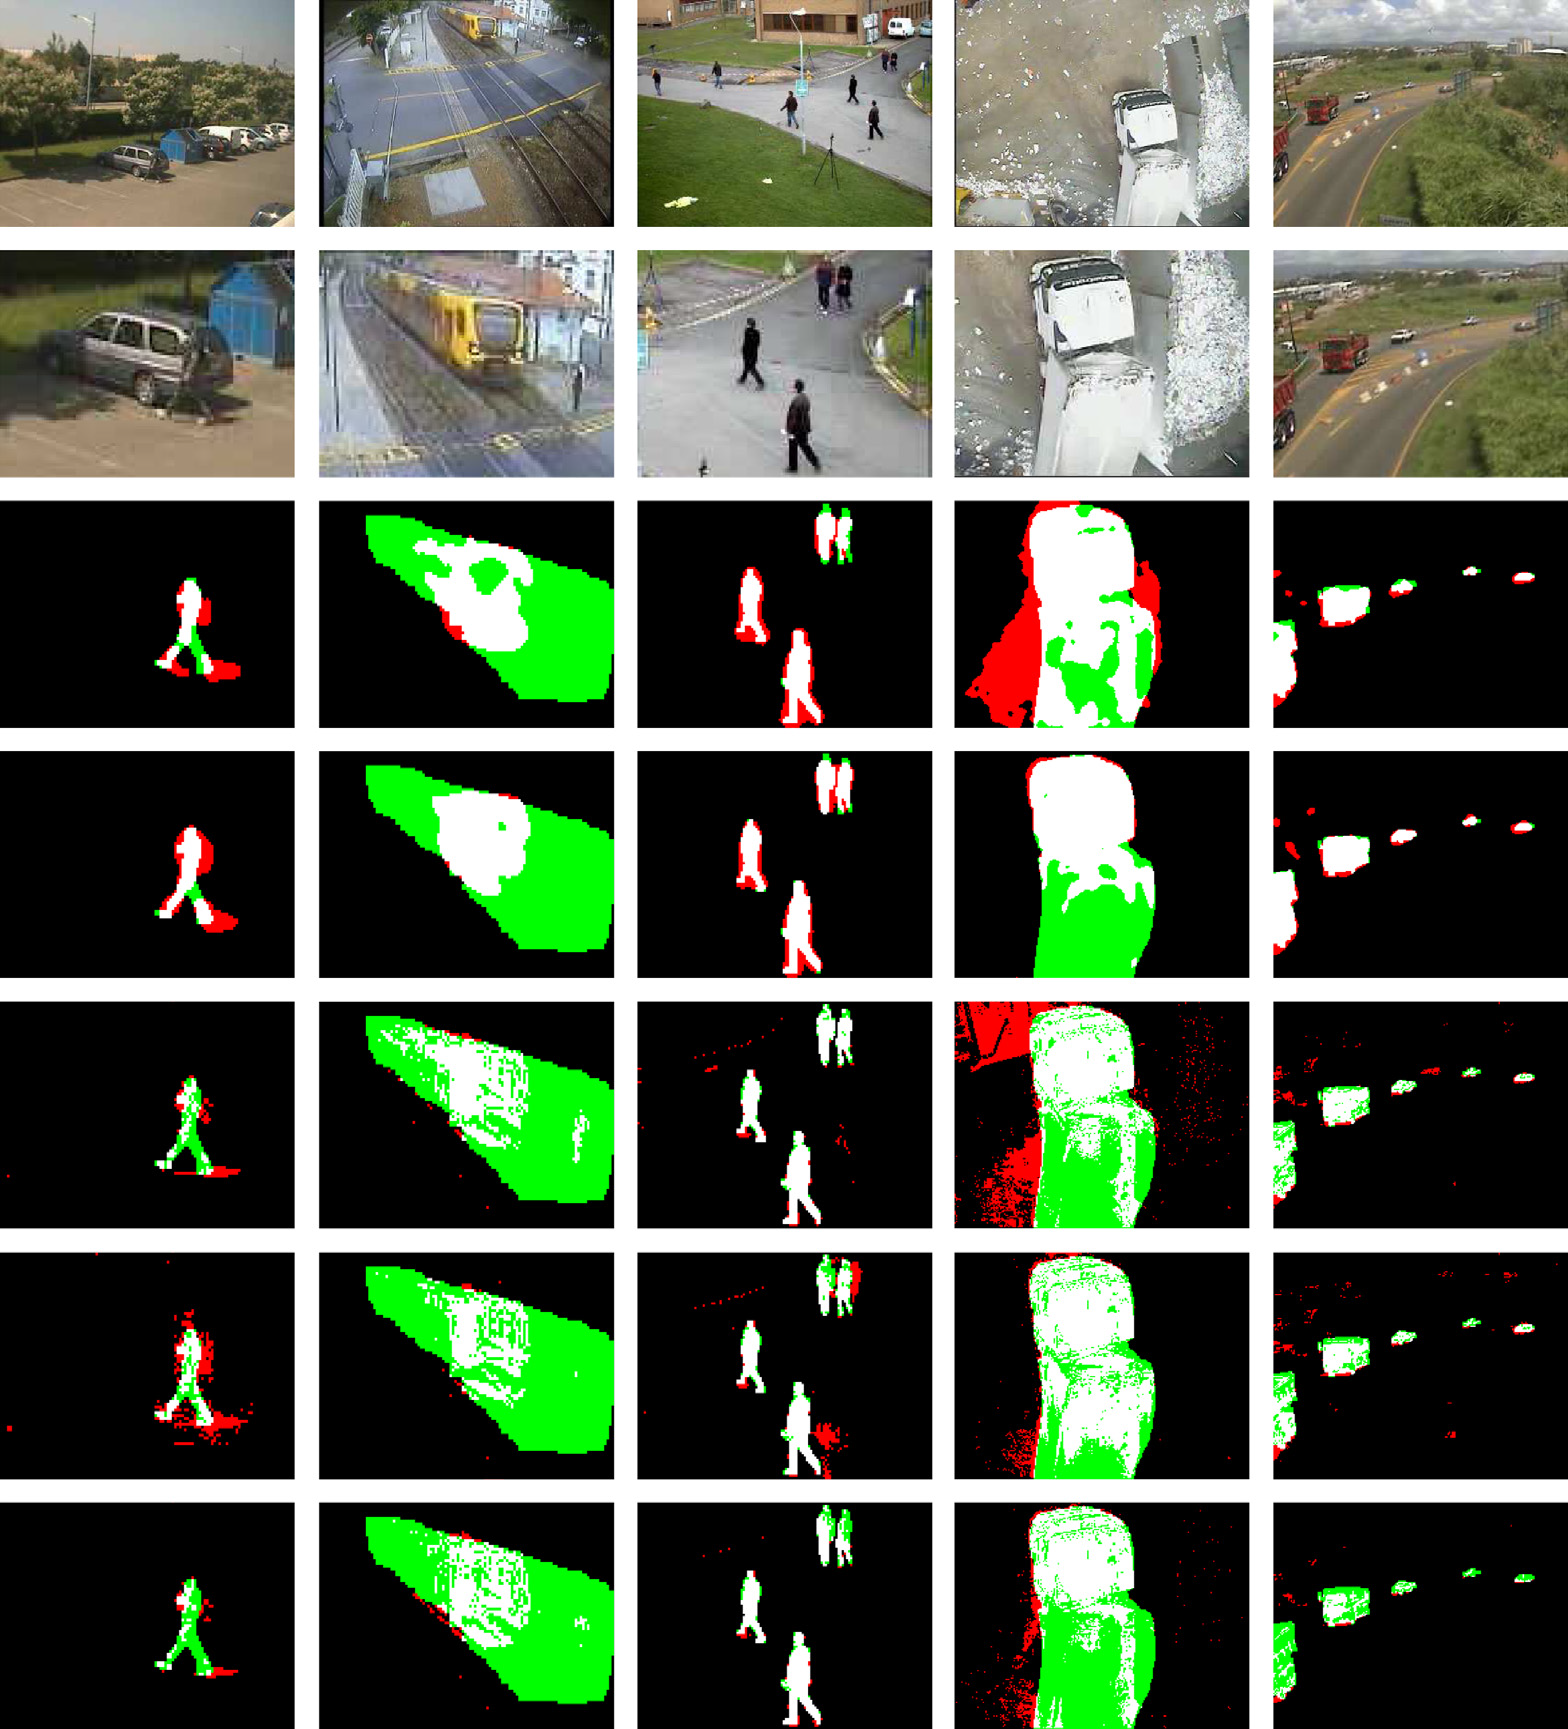
\includegraphics[width=0.9\columnwidth]{bgsreview}
  \caption{Foreground masks obtained from 5 different background subtraction algorithms from real world videos (sourced from \cite{bgs:article}). Images from the first to last row are the input frame, region of interest zoomed in, PBAS, MultiLayerBGS, LBAdaptiveSOM, DPWrenGABGS and MixtureOfGaussianV1BGS algorithms. For the colours, TP pixels are in white, TN pixels are in black, FP pixels are in red, and FN pixels are in green.}
  \label{bgsreview}
\end{figure}

Unfortunately, the PBAS algorithm is no longer available in the BGSLibrary, it is based on the patented ViBE algorithm \cite{barnich2011vibe} therefore was removed \mdc{due to} patent issues. The ViBE algorithm is a powerful background subtraction algorithm with very fast processing speed, high precision and moderate memory usage, the initial implementation is still available, and existed in early versions of OpenCV implemented with CUDA codes runs on GPU.
%}

\iffalse
\subsection{Optical flow}

Optical flow is another widely used object tracking algorithm, it can be used for detect moving objects as well.

There are 2 types of optical flow algorithms. One is sparse feature set (Lucas-Kanade method \cite{bouguet2001pyramidal}), it evaluates pixel movements around selected feature points, therefore calculates movements of feature points. Another type is dense optical flow (Gunner Farneback's algorithm \cite{farneback2003two}), it evaluates pixel movements for all pixels in the frame.

{\color{red}More descriptions and images?}

By rendering pixel movements in 3 axes computed from dense optical flow as 3 components (RGB) colours, then find out regions with the same colour, sizes and positions of moving objects in the scene can then be determined. However, once an object stopped moving, the optical flow algorithms cannot distinguish the object from background any longer.
\fi

\section{Object tracking algorithms}
\label{bg:tracking}

\subsection{Connected component analysis}
\label{blob}

After \mdc{obtaining} the foreground object mask by one of the methods described above, it \modc{needs} to be interpreted as distinct objects, so that the geometry properties of each object can then be retrieved.

Connected component analysis, or connected component labelling, is used for detecting regions that are \moda{different} in some properties, such as colour or brightness. Such a region is also called a blob, which can be the possible presence region of an independent object if applied to the foreground masks. It is very useful to extract parameters such as shape, size and location of the object afterwards.

There are open source blob detection libraries available, such as the simple blob detector came with OpenCV \cite{opencv:blob}, and the cvBlob library \cite{cvblob}. \fref{cvblob} shows an example of tracking blobs by using the cvBlob library.

%{\color{red}Images}

\begin{figure}[H]
  \centering
  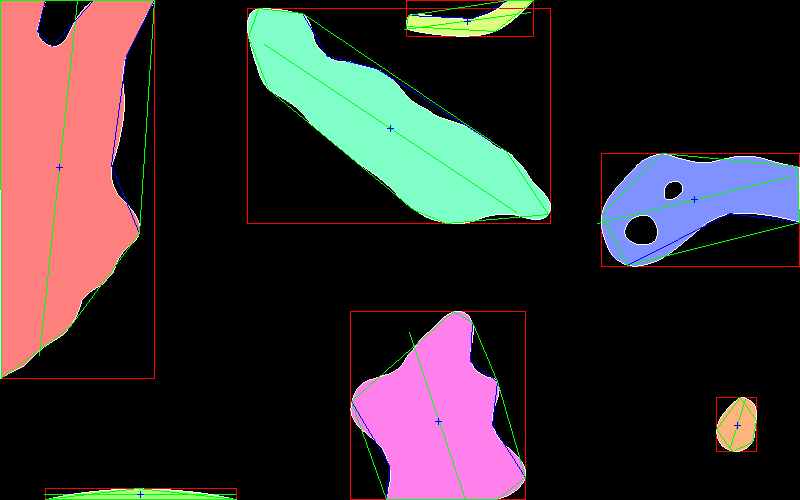
\includegraphics[width=0.7\columnwidth]{cvblob}
  \caption{Tracking blobs with the cvBlob library with bounding shapes, bounding rectangles and blob centres shown (sourced from \cite{cvblob}).}
  \label{cvblob}
\end{figure}

After \modc{determining} the bounding shape, or region of interest (ROI) of an object, the object can then be tracked between adjacent frames by matching the blobs based on similarity in colour and shape or relative position. Movement parameter such as velocity and acceleration may also be obtained by physical modelling.

\subsection{Meanshift and CAMshift}

Meanshift \cite{fukunaga2013introduction} is an algorithm \mdc{which} can be used to track the movement of a fixed size ROI window between adjacent frames. To accomplish this, histogram back projection \mdc{needs} to be applied first to the new frames, which converts the frame to a probability image of each pixels \mdc{belonging} to the target model. Then the meanshift algorithm will be applied to find the peak of probability distribution of the target model. It was implemented within the OpenCV library \cite{opencv:camshift}. \fref{bg:ms:meanshift} shows an example tracking result.

% {\color{red}Images}

Continuously Adaptive Meanshift (CAMshift) \cite{bradski1998computer} is an algorithm based on the Meanshift algorithm, that can handle target object size changing and rotation by iterating over the ROI to find the most suitable configuration. \moda{This algorithm was used by lots of researches for tracking purpose \cite{chu2007object}\cite{xu2012moving}\cite{nouar2006improved}. It was also implemented in the OpenCV library \cite{opencv:camshift}.}. \fref{bg:ms:camshift} shows an example tracking result, \mdc{compared} to the Meanshift algorithm tracking (\fref{bg:ms:meanshift}), it can resize and rotate ROI automatically.

\begin{figure}[H]
  \centering
  \subfigure [] {
    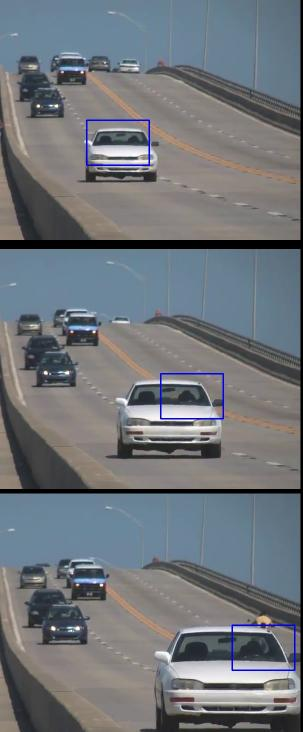
\includegraphics[width=0.3\columnwidth]{meanshift_result}
    \label{bg:ms:meanshift}
  }
  \subfigure [] {
    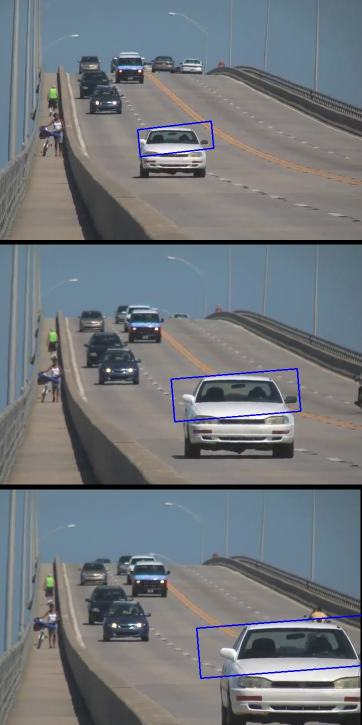
\includegraphics[width=0.35\columnwidth]{camshift_result}
    \label{bg:ms:camshift}
  }
  \caption{Meanshift and CAMshift tracking examples (sourced from \cite{opencv:camshift}). \subref{bg:ms:meanshift} shows the Meanshift tracking, \subref{bg:ms:camshift} shows the CAMshift tracking.}
  \label{bg:ms}
\end{figure}

%{\color{red}Images}

\subsection {Optical flow}

%By evaluating pixel movements of feature points inside ROI, the speeds of moving objects projected onto camera sensor can be determined.

Optical flow is another widely used object tracking algorithm that evaluates pixel moving around feature points, by assuming neighbouring pixels will have similar motion as the feature points. Although it can also be used for detecting moving objects by considering regions of points with the same motion as one moving object, once the object stopped moving, the optical flow algorithms cannot distinguish the object from background any longer. Therefore it is mainly used for object tracking rather than detection.

There are 2 types of optical flow algorithms. One is sparse feature set (Lucas-Kanade method \cite{bouguet2001pyramidal}), it estimates pixel movements around selected feature points. To determine feature points, OpenCV implemented a good features to track \cite{shi1994good} algorithm to find the strongest corners in an image. After that, by moving the feature points according to the movements computed, the object can be tracked across sequence of video frames, as shown \mdc{in} \fref{bg:of:opticalflow_lk}.

Another type is dense optical flow (Gunner Farneback's algorithm \cite{farneback2003two}), it evaluates pixel movements for all points in the frame. \fref{bg:of:opticalfb} shows the result from a dense optical flow tracking scene by rendering movements in 3 axes as red, green and blue components respectively.

\begin{figure}[H]
  \centering
  \subfigure [] {
    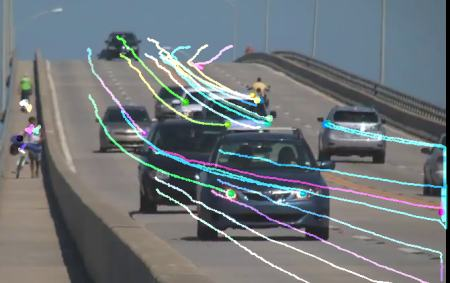
\includegraphics[width=0.3\columnwidth]{opticalflow_lk}
    \label{bg:of:opticalflow_lk}
  }
  \subfigure [] {
    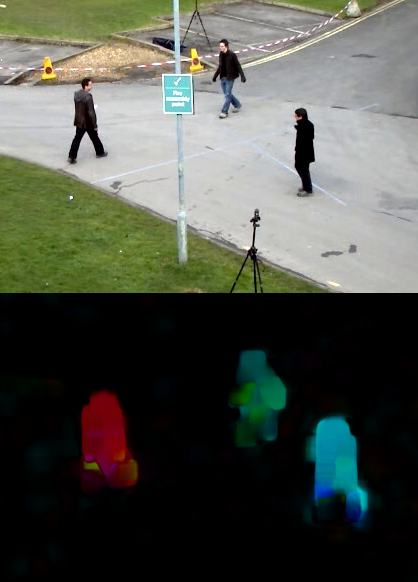
\includegraphics[width=0.3\columnwidth]{opticalfb}
    \label{bg:of:opticalfb}
  }
  \caption{Optical flow example scenes (sourced from \cite{opencv:of}). \subref{bg:of:opticalflow_lk} shows the sparse feature set (Lucas-Kanade method), \subref{bg:of:opticalfb} shows the dense optical flow (Gunner Farneback's algorithm).}
  \label{bg:of}
\end{figure}

% {\color{red}More descriptions and images?}

% {\color{red}Images}

\section{Object recognition}

Object recognition can also be developed by applying different cascade classifiers as described previously in section \ref{sec:bg:cc} to the ROI of the specific object. This process is very computation intensive and time consuming, therefore should be executed as few as possible to \modc{save energy consumption}. \moda{For example, only execute object recognition once the object first enters the sense, or execute to the frame with the maximum visible size of the target object.}

\section{Automatic feedback control}

\mdc{There are researches} about energy-efficient object detection by utilising hardware-level operations \cite{casares2011energy}. \modc{This research \cite{casares2011energy}} had achieved energy consumption reduction by $54.136\%$. However, it was done on a very different and limited platform, based on a very limited algorithm, possible to extend to algorithms with more general usage.

\section{Sample video datasets}

There are sample video datasets proposed for testing, evaluating and comparing computer vision algorithms, specifically background subtraction algorithms. The resolutions are $320 \times 240$ typically, up to about $720 \times 480$, with frame rates of $30$ frames per second (FPS) mostly.

For example, ChangeDetection.NET(CDNET) \cite{goyette2012changedetection} and Background Models Challenge \cite{vacavant2012benchmark} provides realistic camera-captured videos with lots of diverse sets of scenarios and high quality ground truth masks, while Stuttgart Artificial Background Subtraction Dataset \cite{brutzer2011evaluation} was using 3D models and ray tracing technology to generate artificial but realistic videos of typical video surveillance scenarios.

%% ----------------------------------------------------------------
%% HWSW.tex
%% ----------------------------------------------------------------
\chapter{Platforms and interfaces}

This section describes the hardware platforms and software interfaces used to accomplish this project.

\section{Hardware platforms}

\subsection{Embedded host platform}

The Jetson Tegra K1 embedded development platform \cite{NVIDIA:tk1} featuring a 2.32GHz quad-core ARM CPU and a CUDA-enabled Tegra GPU, introduced by NVIDIA, was used in this project. The fact that it is an embedded platform enables easy power consumption analysis, a rich set of peripherals interfaces exposed enables direct control and interfacing a camera module and it is powerful enough to compile programs and execute complex computer vision algorithms.

\subsection{Camera module}
\label{hwsw:camera}

Specific camera module to be used was not determined yet at the time this progress report was written, but it would be a high resolution camera module from OmniVision \cite{ovt} that can be easily interfaced and directly controlled with the peripheral interfaces on the Jetson TK1 platform. A Linux kernel module driver probably need to be developed in order to control the camera parameters and operations from program running in user space.

\subsection{Testing platform}

The computer vision algorithms that are platform and hardware independent were firstly tested on a generic laptop with built in webcam running Microsoft Windows, mainly because it was easier for user interaction and parameter tuning.

\section{Software interfaces}

\subsection{Embedded operating system}

Ubuntu Linux distribution version 14.04.1 LTS was used on the platform, installed directly from the file system image provided by NVIDIA. Linux is great for this project because it is fully configurable, so that operating system overheads can be reduced to minimum by disabling unused services and even the graphical desktop environment. Also most Linux operations could be done through just command line interface, perhaps via a SSH shell access, therefore programming and control the platform could be done anywhere with internet connection, which is very convenient.

\subsection{Computer vision API}

OpenCV \cite{opencv} was used to implement the algorithms, due to its cross platform adaptability, easy to use and large number of existing algorithms ready for use and investigation. Furthermore, the OpenCV library for Jetson platform developed by NVIDIA was further optimised, can provide 2x-5x speed up compare to regular OpenCV \cite{NVIDIA:perf}. The OpenCV GPU module based on NVIDIA CUDA was also available, can provide 5x-20x speed up. These optimisations can reduce computation time dramatically, thus lower the power consumption further.

%% ----------------------------------------------------------------
%% Implement.tex
%% ----------------------------------------------------------------
\chapter{Implementation}

There were lots of different algorithms existing for object detection and tracking. Some of those algorithms were investigated in this project in order to identify a set of suitable algorithms that were both accurate and efficient enough to analysis video stream from camera in real-time.

\section{Background subtraction}

Being able to detect objects in a video frame is the first, also the most difficult and important step to do object tracking. This is generally accomplished by separation of foreground objects and background image. Three different object detection methodologies were investigated in this project.

\subsection{Colour based}

Colour can provides enough information of a specific object. For easier analysis of colour information, a hue-saturation-value (HSV) colourspace \cite[p.~301]{colourspace} representation converted from the original RGB colourspace is usually used, because it would be easier to filter a range of colour based on hue, saturation and brightness.

A simple colour based foreground mask can be generated easily by filtering target colour. An simple implementation \cite{MOTBOC.git} of colour filtering object detection algorithm was investigated, as shown in \fref{Figure:MOTBOC}.

\begin{figure}[H]
  \centering
  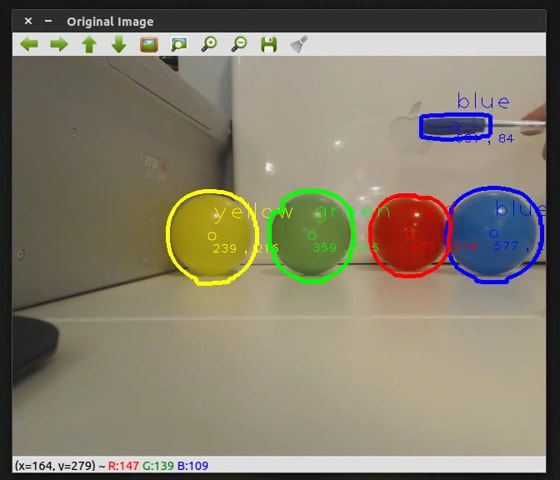
\includegraphics[width=0.6\columnwidth]{MOTBOC}
  \caption{Multi Object Tracking Based on Color (adapted from \cite{MOTBOC.git})}
  \label{Figure:MOTBOC}
\end{figure}

This implementation doesn't require a lot of computation, thus was very fast, could be suitable for robots that are tracking sonething like a single coloured ball or piece of paper, also could be useful for line racing car projects.

However, this implementation is very limited, it can only detects objects with single colour, cannot distinguishes the objects from similar background colour, relies heavily on manually adjusted colour threshold values, and is very sensitive to the variations of colourspaces from different cameras, not very adaptable. A complex environment may also results into lots of undesired detections, as shown in \fref{Figure:MOTBOC_F}.

\begin{figure}[H]
  \centering
  \includegraphics[width=0.6\columnwidth]{"MOTBOC failure"}
  \caption{Simple Multi Object Tracking Based on Color \cite{MOTBOC.git} at a complex environment}
  \label{Figure:MOTBOC_F}
\end{figure}

\subsection{Shape based}

Another important information about an object is its shape. By extracting hard object edges in the scene than apply appropriate shape transformation and filtering algorithms, an object could also be detected based on the shape.

\fref{Figure:circles} shows the image processed by circle detection, based on OpenCV's implementation of Hough Circle Transform \cite{opencv:hough_circle}. The coin at the top right corner had not been detected, because it actually appears to be a eclipse to the algorithm because of visual perspective.

\begin{figure}[H]
  \centering
  \subfigure [] {
    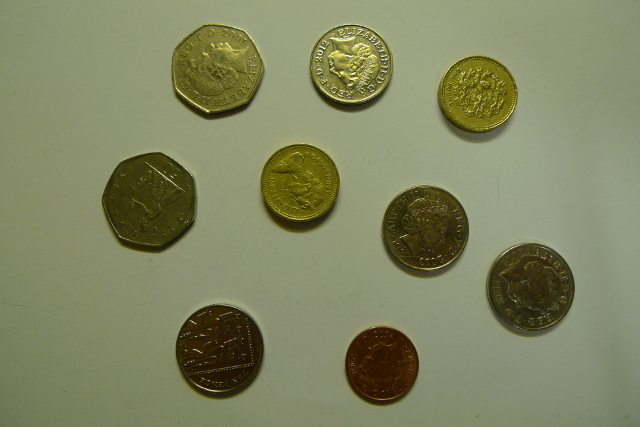
\includegraphics[width=0.45\columnwidth]{simple_original}
    \label{Figure:edges:original}
  }
  \subfigure [] {
    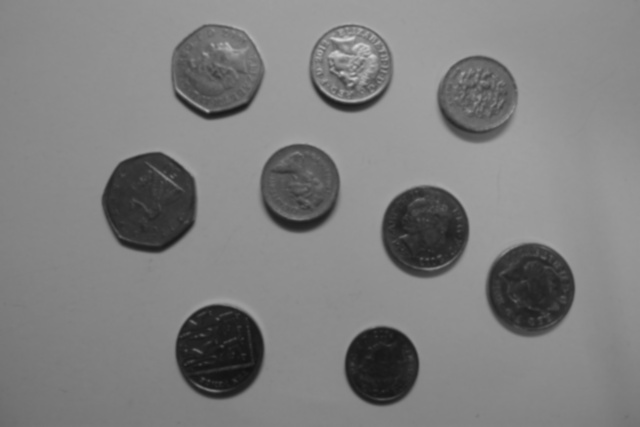
\includegraphics[width=0.45\columnwidth]{simple_blur}
    \label{Figure:edges:blur}
  }
  \subfigure [] {
    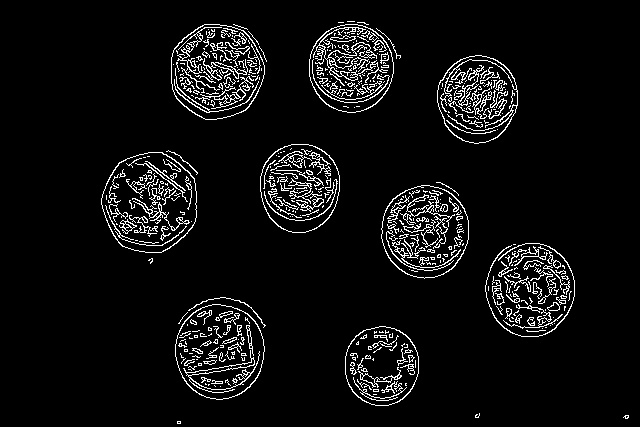
\includegraphics[width=0.45\columnwidth]{simple_edges}
    \label{Figure:edges:edges}
  }
  \subfigure [] {
    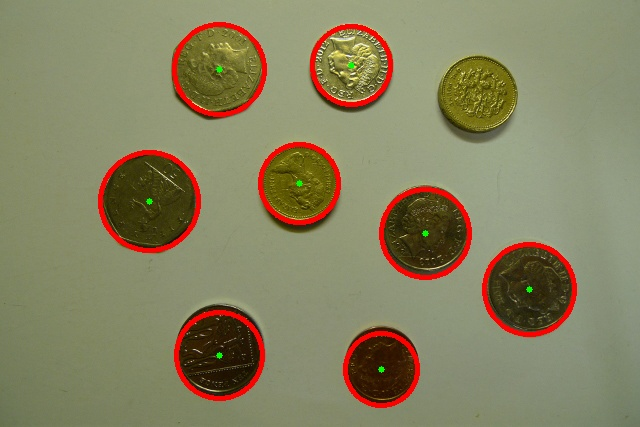
\includegraphics[width=0.45\columnwidth]{simple_circles}
    \label{Figure:edges:circles}
  }
  \caption{Circle detection. \subref{Figure:edges:original} The original image, \subref{Figure:edges:blur} image converted to gray scale and blurred, \subref{Figure:edges:edges} edges detected, \subref{Figure:edges:circles} circles detected}
  \label{Figure:circles}
\end{figure}

\subsection{Cascade Classifier}

Cascade classifier \cite{cascade} is another widely used technique for object detection. It concatenates several classifiers detecting different object features to recognise objects, and it can be trained both positively and negatively to improve accuracy. It was usually used for object classify, for example recognise human and different classes of vehicles in a single frame.

The OpenCV's cascade classifier implementation \cite{opencv:cc} of face and eye detection was investigated as shown in \fref{Figure:cc_face}.

\begin{figure}[H]
  \centering
  \includegraphics[width=0.6\columnwidth]{"CC face"}
  \caption{Face and eye detection cascade classifiers, detected face was circled by pink, whereas detected eyes were circled by blue}
  \label{Figure:cc_face}
\end{figure}

Noticeable frame rate drop and latency was experienced when using the cascade classifier implementation on the testing platform, suggests it was not a fast enough algorithm for real-time object tracking application. In addition, multiple classifier definition files were required for detecting different kinds of objects, or even different perspectives of the same object, which would require lots of computations.

\subsection{Motion based}

By differenceing current frame and previous frames, it is also possible to detects moving objects efficiently. The BGSLibrary \cite{bgslibrary} is specifically developed for this purpose, it offers 37 different background substraction algorithms using OpenCV, published under GNU GPL v3 license.

The article \cite{bgs:article} reviewed the algorithms available in the BGSLibrary, ranked 5 algorithms as the best methods for accuracy. Except the Pixel-Based Adaptive Segmenter (PBAS) algorithm which was removed due to patent issues, the other 4 algorithms listed in \tref{Table:bgs} were investigated in this project.

\begin{table}[H]
  \centering
  \begin{tabular}{cc}
  \toprule
  \textbf{Method ID} & \textbf{Method name}\\
  \midrule
  MultiLayerBGS & Multi-Layer BGS \\
  MixtureOfGaussianV1BGS & Gaussian Mixture Model \\
  LBAdaptiveSOM & Adaptive SOM \\
  DPWrenGABGS & Gaussian Average \\
  \bottomrule
  \end{tabular}
  \caption{Background substraction algorithms investigated (adapted from \cite{bgslibrary})}
  \label{Table:bgs}
\end{table}

\fref{Figure:bgs_frame} shows the foreground masks obtained from those 4 algorithms through 2 sample frame sequences available with the BGSLibrary \cite{bgslibrary}.

\begin{figure}[H]
  \centering
  \includegraphics[width=0.24\columnwidth]{bgs_frame/MultiLayerBGS/input}
  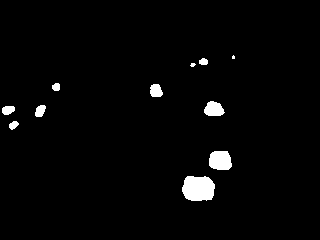
\includegraphics[width=0.24\columnwidth]{bgs_frame/MultiLayerBGS/mask}
  %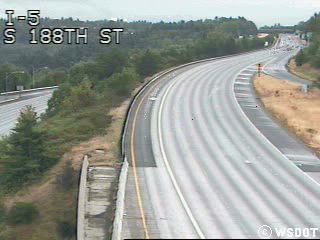
\includegraphics[width=0.32\columnwidth]{bgs_frame/MultiLayerBGS/bkgmodel}
  \includegraphics[width=0.24\columnwidth]{bgs_video/MultiLayerBGS/input}
  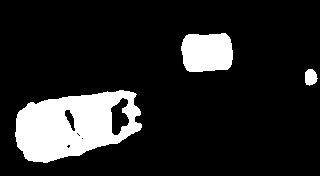
\includegraphics[width=0.24\columnwidth]{bgs_video/MultiLayerBGS/mask}

  \includegraphics[width=0.24\columnwidth]{bgs_frame/MixtureOfGaussianV1BGS/input}
  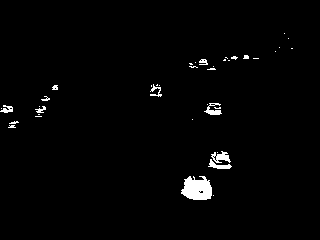
\includegraphics[width=0.24\columnwidth]{bgs_frame/MixtureOfGaussianV1BGS/mask}
  \includegraphics[width=0.24\columnwidth]{bgs_video/MixtureOfGaussianV1BGS/input}
  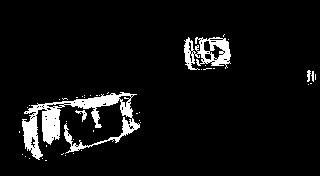
\includegraphics[width=0.24\columnwidth]{bgs_video/MixtureOfGaussianV1BGS/mask}
  %
\includegraphics[width=0.32\columnwidth]{na}

  \includegraphics[width=0.24\columnwidth]{bgs_frame/LBAdaptiveSOM/input}
  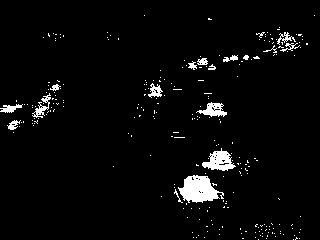
\includegraphics[width=0.24\columnwidth]{bgs_frame/LBAdaptiveSOM/mask}
  \includegraphics[width=0.24\columnwidth]{bgs_video/LBAdaptiveSOM/input}
  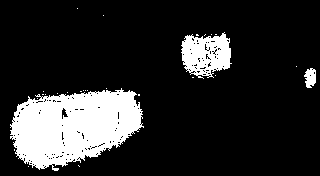
\includegraphics[width=0.24\columnwidth]{bgs_video/LBAdaptiveSOM/mask}
  %
\includegraphics[width=0.32\columnwidth]{na}

  \includegraphics[width=0.24\columnwidth]{bgs_frame/DPWrenGABGS/input}
  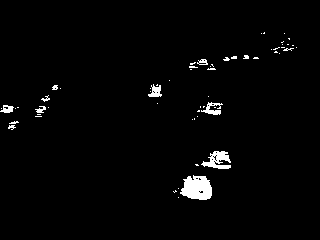
\includegraphics[width=0.24\columnwidth]{bgs_frame/DPWrenGABGS/mask}
  \includegraphics[width=0.24\columnwidth]{bgs_video/DPWrenGABGS/input}
  
\includegraphics[width=0.24\columnwidth]{bgs_video/DPWrenGABGS/mask}
  %
\includegraphics[width=0.32\columnwidth]{na}
  \caption{Results obtained from background substraction algorithms. From left to right column: input sample 1, foreground mask obtained, input sample 2, foreground mask obtained. From top to bottom row: MultiLayerBGS, MixtureOfGaussianV1BGS, LBAdaptiveSOM and DPWrenGABGS.}
  \label{Figure:bgs_frame}
\end{figure}

It can be seen from \fref{Figure:bgs_frame} that MultiLayerBGS gave the best foreground masks, but it was also the slowest algorithm on the testing platform.

\section{Movement tracking}

After obtained the foreground object mask, they need to be interpreted as objects, then the object can be detected and tracked based on its position.

\subsection{Connected component analysis} \label{blob}

Connected component analysis, or Connected component labeling, is used for detecting connected regions (blobs). A blob detector can be used to mark and labeling individual objects from the foreground mask, therefore obtain parameters such as size, position and orientation of the object. Afterwards, by comparing nearby objects from previous frames, the objects can be tracked, and movement parameter such as velocity and acceleration can then be obtained by physical modelling.

There were also lots of free and open source blob detection libraries available, e.g. the simple blob detector came with OpenCV \cite{opencv:blob}, cvBlob library \cite{cvblob}.

This was not yet implemented at the time this progress report was written.

\subsection{Continuously Adaptive Meanshift}

Continuously Adaptive Meanshift (CAMshift) \cite{bradski1998computer} is a technique used to track a region of interest (ROI) in continuous frame sequences. It is based on Meanshift algorithm, which only track a fixed size ROI window, whereas CAMshift can handle target resize and rotation. In order to determine the ROI for CAMshift, the blob detector as described in Section \ref{blob} can also be used. This algorithm can also be easily implemented using OpenCV \cite{opencv:camshift}, and was used by lots of researches such as \cite{chu2007object}, \cite{xu2012moving} and \cite{nouar2006improved}.

This was not yet implemented at the time this progress report was written.

%\chapter{Project management}

\section{Risk management}

\begin{table}[!htb]
  \centering
  \begin{tabular}{|p{0.16\columnwidth}|c|c|p{0.42\columnwidth}|}
  \hline
  \textbf{Risk (event)} & \textbf{Likelihood} & \textbf{Impact} & \textbf{Action} \\ \hline
  Camera module failure & Low & High & Buy redundant camera modules. \\ \hline
  Jetson board failure & Low & High & Find another one, or find alternative ways to continue the project. \\ \hline
  Test facilities not available & Low & Medium & Check in advance. \\ \hline
  ECS file storage server is slow & Medium & Medium & Use my own laptop. \\ \hline
  Supervisor is away at meeting & High & Low & Read literatures, continue implementations. \\ \hline
  Unexpected accident or illness & Low & High & Try to avoid. Have multiple backups. \\ \hline
  Unable to implement camera driver & Medium & High & Find easy alternatives, or read frames from video files. \\ \hline
  Unable to implement some algorithms & Medium & High & Find easy alternatives. \\ \hline
  \end{tabular}
  \caption{Risk assessment}
  \label{man:risk}
\end{table}

\subsection{Board failure}

During the second semester, the Jetson board accidentally failed on 3rd, Match. I was probing a current sensor resistor on the board, then unintentionally short circuited the 12V power rail to the 3.3V power rail. Although the CPU, GPU cores and some peripheral interfaces survived, two of the power rails were still in short circuit condition and cannot be easily diagnosed. As a result, USB, Ethernet and HDMI interfaces were not functioning. The board can only be controlled through a UART interface, with a voltage level converter chip. Power consumption analysis would also be affected by the two short circuited power rails.

I quickly transferred the algorithm development to a general purpose computer to continue working on it. This could be done only because all the source codes were regularly backed up on the git server. Having recognised that the board is only essential for power consumption modelling, reasonable results were still possible even without the board. The algorithms can run on a general computer, most analyses are still possible. Finally, after some negotiation with my supervisor, another board was available for use, the development was then transferred to the new board.

\section{Time management}

The topic of project changed once during week 7 in semester 1. The previous topic (\aref{Appendix:brief_prev}) was about reducing power consumption for algorithms that are utilising General Purpose GPU (GPGPU) technique, by adaptively controlling calculation precision. The NVIDIA Jetson TK1 development platform was decided to be used in this project. However, after investigated into the topic and experimented with some algorithms, the purposed precision control did not contribute significant impact on computation quality. Not much power saving would be possible to be made.

Therefore, I decided to change the project topic. The current project topic (\aref{Appendix:brief}) was quickly determined. The same hardware platform was still used, so that the time invested in the previous project was not wasted. Therefore, I was able to quickly catch up with the progress.

The Gantt chart was also changed due to project topic changing, as shown in \fref{gantt_prev} and \fref{gantt_rev}. The time invested for previous project topic was treated as background reading. \fref{gantt} shows the actual time spend on each of the items.

\begin{figure}[H]
  \centering
  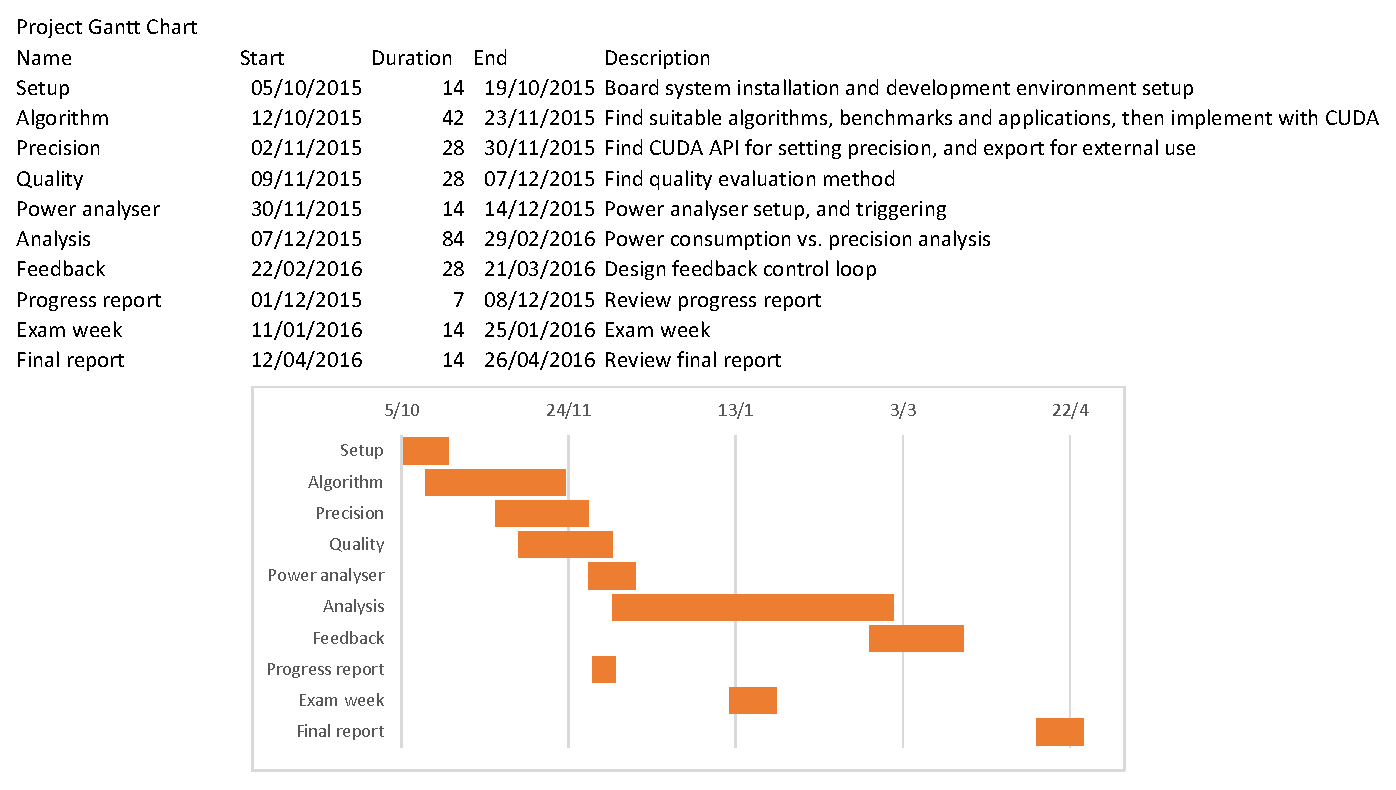
\includegraphics[width=\columnwidth]{Gantt_previous}
  \caption{Previous Gantt chart}
  \label{gantt_prev}
\end{figure}

\begin{figure}[H]
  \centering
  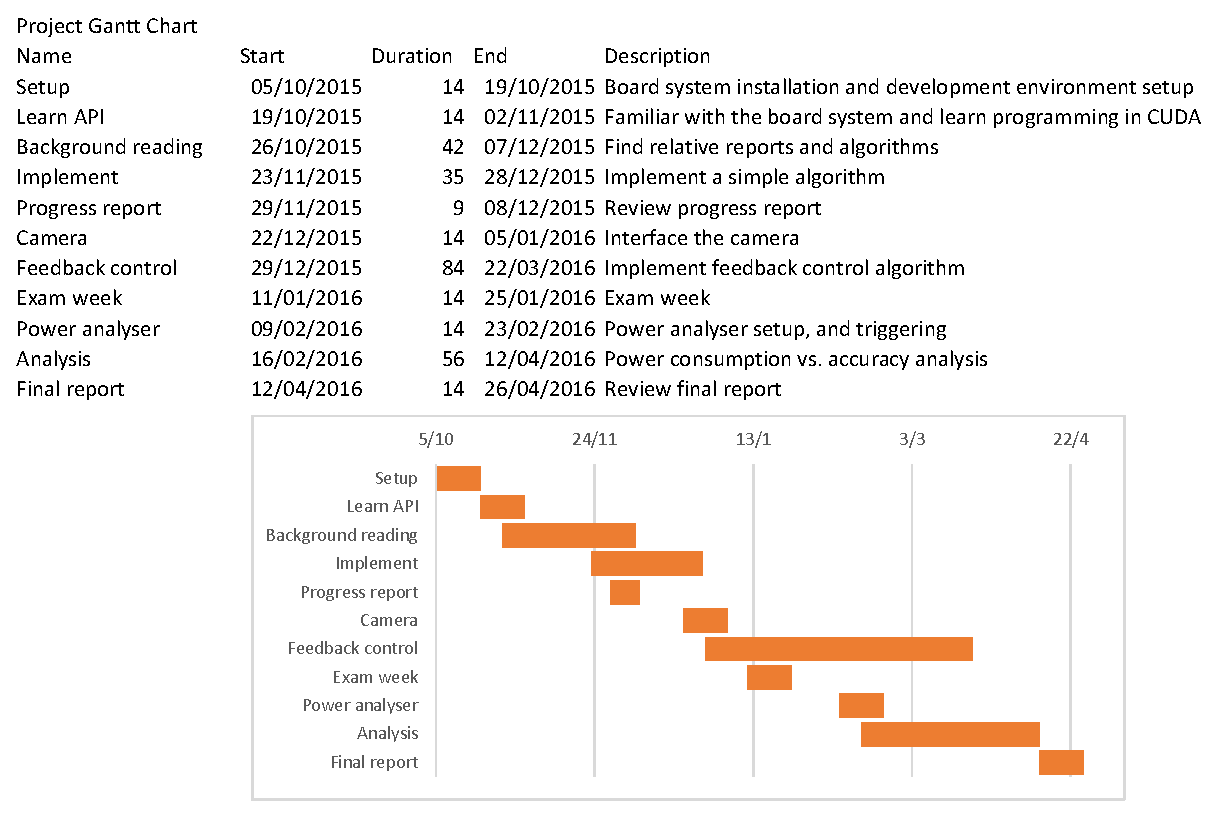
\includegraphics[width=\columnwidth]{Gantt_interim}
  \caption{Revised Gantt chart}
  \label{gantt_rev}
\end{figure}

\begin{figure}[H]
  \centering
  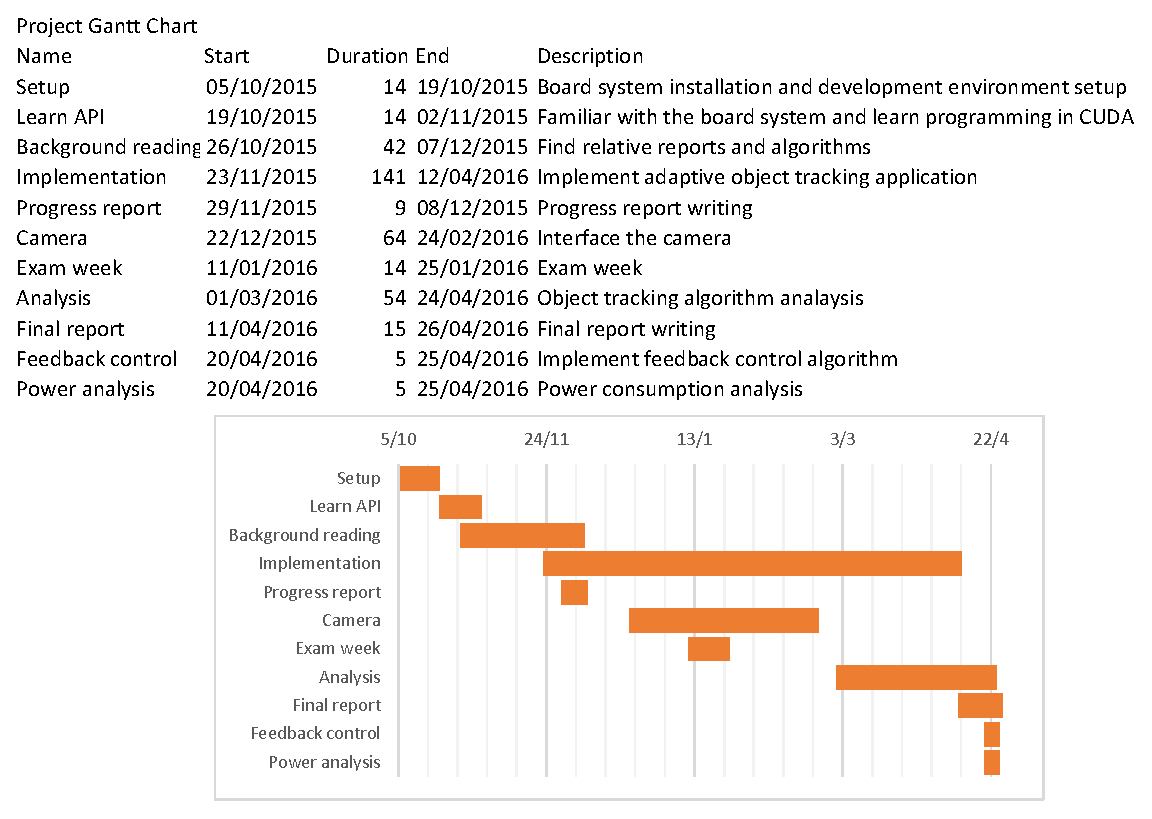
\includegraphics[width=\columnwidth]{Gantt}
  \caption{Actual time usage}
  \label{gantt}
\end{figure}

\section{Backing up}

%Source code management.
%Documents and materials.

The git version control system \cite{git} was used in this project. It has the feature that allows multiple users collaborate on the same repository. However, this is an individual project, git was used purely for backing up source code version history and synchronisation between multiple devices. Well-known git hosting website GitHub \cite{github} and university's SourceKettle server \cite{sourcekettle} were used for multiple backups.

All documents, background literals and materials used by the project were backed up using Microsoft's OneDrive service.

%\section{Remaining work}

%\begin{itemize}
%  \item Movement tracking based on blob detection (Section \ref{bg:tracking}, \ref{impl:tracking}).
%  \item A camera module need to be ordered and interfaced.
%  \item Automatic frame rate reduction based on tracking result.
%  \item Hardware downsampling and cropping based on ROI.
%  \item If time allows, energy-efficient object recognition may be implemented.
%\end{itemize}

\appendix
%%% ----------------------------------------------------------------
%% AppendixA.tex
%% ---------------------------------------------------------------- 
\chapter{Stuff} \label{Chapter:Stuff}
The following gets in the way of the text....


\backmatter
\bibliography{Reference}
\end{document}
%% ----------------------------------------------------------------
